\documentclass[aps,prb,twocolumn,superscriptaddress,floatfix,longbibliography]{revtex4-2}

\usepackage[utf8]{inputenc}
\usepackage[spanish]{babel}
\usepackage{graphicx}
\usepackage{amsmath}
\usepackage{subcaption}
\usepackage{wrapfig} 
\usepackage[export]{adjustbox}

\usepackage{amsmath,amssymb} % math symbols
\usepackage{bm} % bold math font
\usepackage{graphicx} % for figures
\usepackage{comment} % allows block comments
\usepackage{textcomp} % This package is just to give the text quote '
%\usepackage{ulem} % allows strikeout text, e.g. \sout{text}

\usepackage[spanish]{babel}

\usepackage{enumitem}
\setlist{noitemsep,leftmargin=*,topsep=0pt,parsep=0pt}

\usepackage{xcolor} % \textcolor{red}{text} will be red for notes
\definecolor{lightgray}{gray}{0.6}
\definecolor{medgray}{gray}{0.4}

\usepackage{hyperref}
\hypersetup{
colorlinks=true,
urlcolor= blue,
citecolor=blue,
linkcolor= blue,
bookmarks=true,
bookmarksopen=false,
}

% Code to add paragraph numbers and titles
\newif\ifptitle
\newif\ifpnumber
\newcounter{para}
\newcommand\ptitle[1]{\par\refstepcounter{para}
{\ifpnumber{\noindent\textcolor{lightgray}{\textbf{\thepara}}\indent}\fi}
{\ifptitle{\textbf{[{#1}]}}\fi}}
%\ptitletrue  % comment this line to hide paragraph titles
%\pnumbertrue  % comment this line to hide paragraph numbers

% minimum font size for figures
\newcommand{\minfont}{6}

% Uncomment this line if you prefer your vectors to appear as bold letters.
% By default they will appear with arrows over them.
% \renewcommand{\vec}[1]{\bm{#1}}

%Cambiar Cuadros por Tablas y lista de...
%\renewcommand{\listtablename}{Índice de tablas}
\renewcommand{\tablename}{Tabla}
\renewcommand{\date}{Fecha}

\graphicspath{ {C:/Users/lupam/OneDrive/Escritorio/GitHub/Metodos_Num_Fluidos_I/Guias/Guia_2/Ejercicio_4/Programa/graficos} } %Para importar imágenes desde una carpeta


\usepackage[bottom]{footmisc} %para que las notas al pie aparezcan en la misma página



\begin{comment}

%Comandos de interés:

* Para ordenar el documento:
\section{Introducción}
\section{\label{sec:Formatting}Formatting} %label para luego hacer referencia a esa sección

\ptitle{Start writing while you experiment} %pone nombre y título al documento dependiendo de si en el header están los comandos \ptitletrue y \pnumbertrue

* Ecuaciones:
\begin{equation}
a^2+b^2=c^2 \,.
\label{eqn:Pythagoras}
\end{equation}

* Conjunto de ecuaciones:
\begin{eqnarray}
\label{eqn:diagonal}
\nonumber d & = & \sqrt{a^2 + b^2 + c^2} \\
& = & \sqrt{3^2+4^2+12^2} = 13
\end{eqnarray}

* Para hacer items / enumerar:
\begin{enumerate}
  \item
\end{enumerate}

\begin{itemize}
  \item
\end{itemize}

* Figuras:
\begin{figure}[h]
    \includegraphics[clip=true,width=\columnwidth]{pixel-compare}
    \caption{}
     \label{fig:pixels}
\end{figure}

* Conjunto de figuras:
(no recuerdo)


* Para hacer referencias a fórmulas, tablas, secciones, ... dentro del documento:
\ref{tab:spacing}

* Para citar
Elementos de .bib
\cite{WhitesidesAdvMat2004}
url
\url{http://www.mendeley.com/}\\

* Agradecimientos:
\begin{acknowledgments}
We acknowledge advice from Jessie Zhang and Harry Pirie to produce Fig.\ \ref{fig:pixels}.
\end{acknowledgments}

* Apéndice:
\appendix
\section{\label{app:Mendeley}Mendeley}

* Bibliografía:
\bibliography{Hoffman-example-paper}

\end{comment}



\begin{document}

% Allows to rewrite the same title in the supplement
\newcommand{\mytitle}{Laboratorio 2 - ????}

\title{\mytitle}

\author{Pablo Chehade \\
    \small \textit{pablo.chehade@ib.edu.ar} \\
    \small \textit{Métodos Numéricos en Fluidos I, Instituto Balseiro, CNEA-UNCuyo, Bariloche, Argentina, 2022} \\}


\begin{abstract}

Se estudiaron métodos numéricos para resolver problemas de valores iniciales. En particular, se aplicaron los métodos de Euler implícito, Crank-Nicholson, Runge Kutta 4 y Leap-Frog al problema del péndulo simple y el método de Runge Kutta 4 al del péndulo doble. Para todos los casos se estudió el orden de convergencia global del error de fase y el error de amplitud, \textcolor{red}{obteniendo resultados similares a los teóricos?}. También se estudió la sensibilidad del péndulo doble a perturbaciones.

\end{abstract}

\maketitle

\section{Introducción}

\begin{equation}
  1
  \label{eq:pendulo_simple}
\end{equation}

\begin{equation}
  1
  \label{eq:periodo_simple}
\end{equation}


\begin{equation}
  1
  \label{eq:fase_simple}
\end{equation}

\begin{equation}
  1
  \label{eq:amplitud_simple}
\end{equation}


\begin{equation}
  1
  \label{eq:pendulo_doble}
\end{equation}


\begin{equation}
  1
  \label{eq:amplitud_doble}
\end{equation}


\section{Método Numérico}

Ecuación vectorial del péndulo simple
\begin{equation}
  1
  \label{eq:pendulo_simple_vec}
\end{equation}


Ecuación vectorial del péndulo doble
\begin{equation}
  1
  \label{eq:pendulo_doble_vec}
\end{equation}

\begin{equation}
  1
  \label{eq:Euler_implicito}
\end{equation}

\begin{equation}
  1
  \label{eq:Crank_Nicholson}
\end{equation}

\begin{equation}
  1
  \label{eq:Runge_Kutta_4}
\end{equation}

\begin{equation}
  1
  \label{eq:Leap_Frog}
\end{equation}



\section{Resultados y discusión}

\subsection{Péndulo simple}


\begin{figure}[h]
  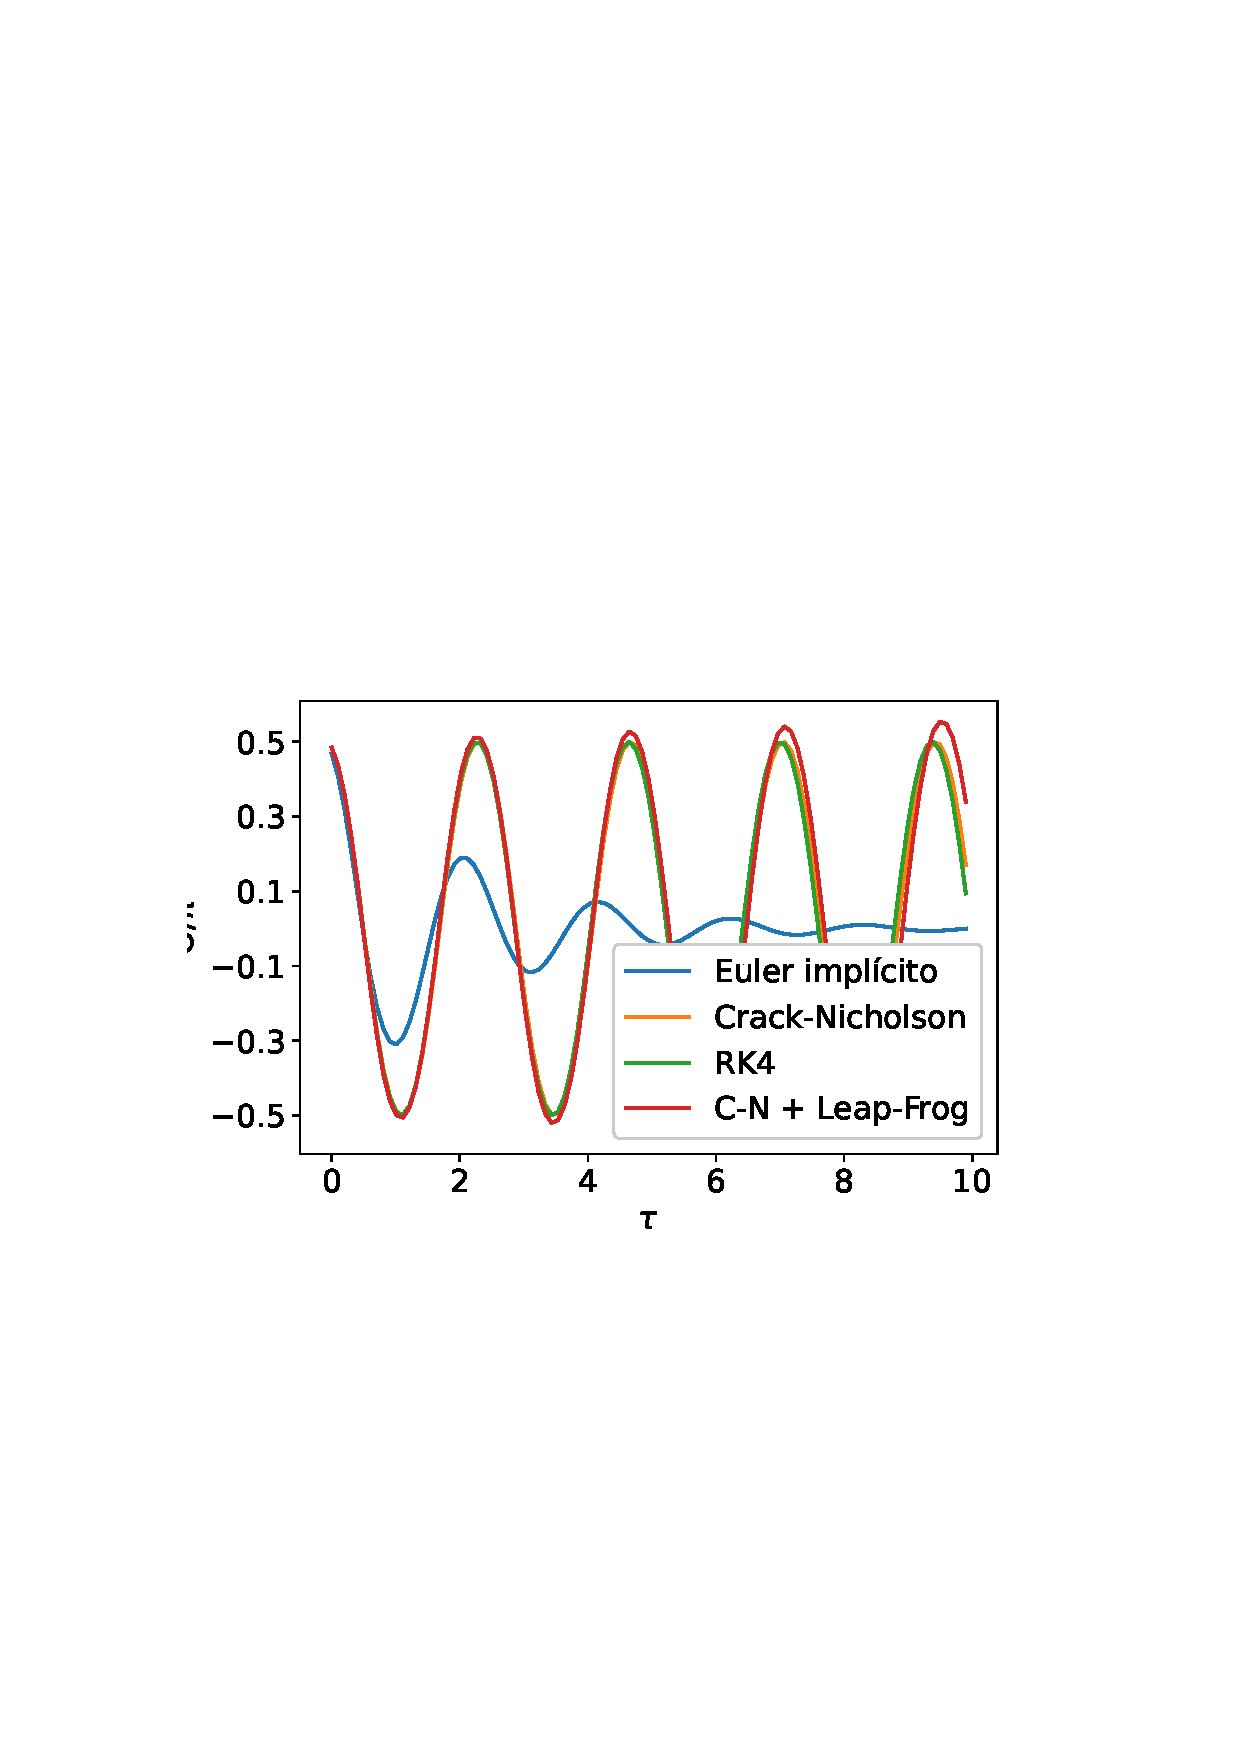
\includegraphics[clip=true,width=\columnwidth]{sol_aprox.pdf}
  \caption{\textcolor{blue}{Solución aproximada por los 4 métodos}}
   \label{fig:sol_aprox}
\end{figure}
% y_ini = [pi/2,0]; #condiciones iniciales
% t_ini = 0;
% n = 99;
% h = 0.1;



\begin{figure}[h]
  \includegraphics[clip=true,width=\columnwidth]{error_amplitud_simple_pi2.pdf}
  \caption{\textcolor{blue}{(b) Error de amplitud para los 4 métodos para tita inicial de pi/2}}
   \label{fig:error_amplitud_simple_pi2}
\end{figure}
% AMPLITUD:
% Orden de convergencia Euler implícito:  0.9372575985568138 +/- 0.01902503308713794
% Orden de convergencia Crack-Nicholson:  5.790183279314054 +/- 0.09070012637078931
% Orden de convergencia RK4:  4.872347720305063 +/- 0.03460069824650806
% Orden de convergencia C-N + Leap-Frog:  2.9552896088114005 +/- 0.04216313986505771


\begin{figure}[h]
  \includegraphics[clip=true,width=\columnwidth]{error_fase_simple_pi2.pdf}
  \caption{\textcolor{blue}{(a) Error de fase para los 4 métodos para tita inicial de pi/2}}
   \label{fig:error_fase_simple_pi2}
\end{figure}
% FASE:
% Orden de convergencia Euler implícito:  0.9094202564952926 +/- 0.03070835705396524
% Orden de convergencia Crack-Nicholson:  1.9609514818114762 +/- 0.019260309080823608
% Orden de convergencia RK4:  3.9163907216640714 +/- 0.02044736620447468
% Orden de convergencia C-N + Leap-Frog:  1.8573616277295897 +/- 0.04875131838369911



\begin{figure}[h]
  \includegraphics[clip=true,width=\columnwidth]{error_amplitud_simple_angulo_bajo.pdf}
  \caption{\textcolor{blue}{(a) Error de fase para los 4 métodos para tita inicial de 10e-4}}
   \label{fig:error_amplitud_simple_angulo_bajo}
\end{figure}
% AMPLITUD:
% Orden de convergencia Euler implícito:  0.9125871407963045 +/- 0.023038374694042806
% Orden de convergencia RK4:  4.940148423340664 +/- 0.023908301779203472
% Orden de convergencia C-N + Leap-Frog:  3.0099767594644535 +/- 0.004694372715781479
% CN tiene error cero creo



\begin{figure}[h]
  \includegraphics[clip=true,width=\columnwidth]{error_fase_simple_angulo_bajo.pdf}
  \caption{\textcolor{blue}{(b) Error de amplitud para los 4 métodos para tita inicial de 10e-4}}
   \label{fig:error_fase_simple_angulo_bajo}
\end{figure}
% FASE:
% Orden de convergencia Euler implícito:  1.969515531340741 +/- 0.02352945286109731
% Orden de convergencia Crack-Nicholson:  1.9315725179531302 +/- 0.031743969584564165
% Orden de convergencia RK4:  4.020308658595079 +/- 0.020460933506094077
% Orden de convergencia C-N + Leap-Frog:  1.9591911569629437 +/- 0.019303222788158225


\subsection{Péndulo doble}

\begin{figure}[h]
  \includegraphics[clip=true,width=\columnwidth]{doble_3CI.pdf}
  \caption{\textcolor{blue}{Solución numérica para las 3 distintas condiciones iniciales}}
   \label{fig:doble_3CI}
\end{figure}

\begin{figure}[h]
  \includegraphics[clip=true,width=\columnwidth]{doble_3CI_difs.pdf}
  \caption{\textcolor{blue}{Diferencias entre las soluciones numéricas a tiempo fijo en función de h}}
   \label{fig:doble_3CI_difs}
\end{figure}

% \begin{figure}[h]
%   \includegraphics[clip=true,width=\columnwidth]{doble_3CI_trayectorias.pdf}
%   \caption{\textcolor{blue}{Trayectorias de las 3 condiciones iniciales}}
%    \label{fig:doble_3CI_trayectorias}
% \end{figure}

% \begin{figure}[h]
%   \includegraphics[clip=true,width=\columnwidth]{doble_error_amplitud.pdf}
%   \caption{\textcolor{blue}{Error de amplitud para todo tiempo}}
%    \label{fig:doble_error_amplitud.pdf}
% \end{figure}

% \begin{figure}[h]
%   \includegraphics[clip=true,width=\columnwidth]{doble_orden_error_amplitud.pdf}
%   \caption{\textcolor{blue}{Orden del error de amplitud}}
%    \label{fig:doble_orden_error_amplitud}
% \end{figure}


\section{Conclusión}




\bibliography{Chehade_guia1.bib}

\end{document}





